\section{Experiments}





We conduct a series of experiments to validate the effectiveness of our proposed data and techniques.
First, we evaluate 
our proposed real-world Stereo4D data mined from VR180 videos on the \method task.
In particular, we compare models that are individually trained with our real-world data and with synthetic data, and we show that our data enables model learning more accurate 3D motion priors (\Sec{motion_eval}). 
Second, we show that our trained model that adapts \duster has strong generalization to in-the-wild images of dynamic scenes, and enables accurate predictions of underlying geometry (\Sec{structure_eval}).




\begin{figure*}[ht]
\vspace{-1em}
    \centering
    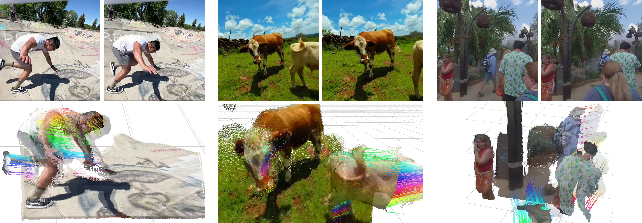
\includegraphics[width=\linewidth]{fig/ours_qualitative.pdf}
    \caption{\textbf{Testing on held out examples from \dataset.} We visualize image pairs and corresponding dynamic 3D point clouds predicted by \method. 
    It recovers accurate 3D shape and complex scene motion for objects such as people breakdancing and cows walking.}
    \label{fig:result-wall-stereo4dtest}
\end{figure*}

\subsection{3D motion prediction} \label{sec:motion_eval}

\noindent \textbf{Baselines and metrics.} 
To evaluate the efficacy of our data paradigm on motion prediction, we primarily compare \method trained on \dataset to the same network trained on a synthetic dataset, PointOdyssey~\cite{zheng2023point}. 
PointOdyssey contains ground truth depth maps and 3D motion tracks rendered from an animation engine;
we supervise the model with this data using the same hyperparameter settings as described above. 
During inference, given two video frames sampled from a video of a dynamic scene, we compare 3D end-point-error (EPE) between ground truth and predicted 3D motion vectors. 
We also 
compute the fraction of 3D points that have motion within 5 cm and 10 cm compared to ground truth ($\delta_{3D}^{0.05}, \delta_{3D}^{0.10}$), following~\cite{teed2021raft3d,wang2024shape}. 
Since our model outputs point clouds up to an unknown scale, we align each prediction with the ground truth through a median scale estimate.
We evaluate models trained on each of these two data sources on a held-out \dataset test-set, as well as on Arial Digital Twin (ADT)~\cite{pan2023aria} data containing scene motion, processed by the TapVid3D benchmark~\cite{koppula2024tapvid3d}. 
As test data, we randomly sample pairs of frames that are at most 30 frames apart from both \dataset and ADT.


 

\begin{table}[!t]
\centering
\footnotesize
\renewcommand{\arraystretch}{0.95}
\renewcommand{\tabcolsep}{2.pt}

\resizebox{\linewidth}{!}{
\begin{tabular}{@{}lcccccc@{}}
\toprule
  & \multicolumn{3}{c}{Stereo4D} & \multicolumn{3}{c}{ADT} \\ 
 
\cmidrule(lr){2-4} \cmidrule(lr){5-7}
 Method & $\text{EPE}_\text{3D}$$\downarrow$&	$\delta_\text{3D}^{0.05}$$\uparrow$ &$\delta_\text{3D}^{0.10}$$\uparrow$& $\text{EPE}_\text{3D}$$\downarrow$&	$\delta_\text{3D}^{0.05}$$\uparrow$ &$\delta_\text{3D}^{0.10}$$\uparrow$  \\ 
\midrule

  \method (PointOdyssey) &0.6191 & 11.61 & 20.25 & 0.3126 & 8.56 & 18.03\\ 
  \method (\dataset) & \textbf{0.1110} & \textbf{65.07 }& \textbf{75.18} & \textbf{0.1231 }& \textbf{51.98} &\textbf{65.20} \\ 
\bottomrule
\end{tabular}
}
\caption{{\bf Synthetic vs.\ Real Training Data.} Compared to synthetic data (PointOdyssey~\cite{zheng2023point}), training on \dataset improves \method's ability to generalize to real-world motion.}
\label{tab:motion_3d_eval}
\end{table}


\begin{figure}[ht]
    \centering
    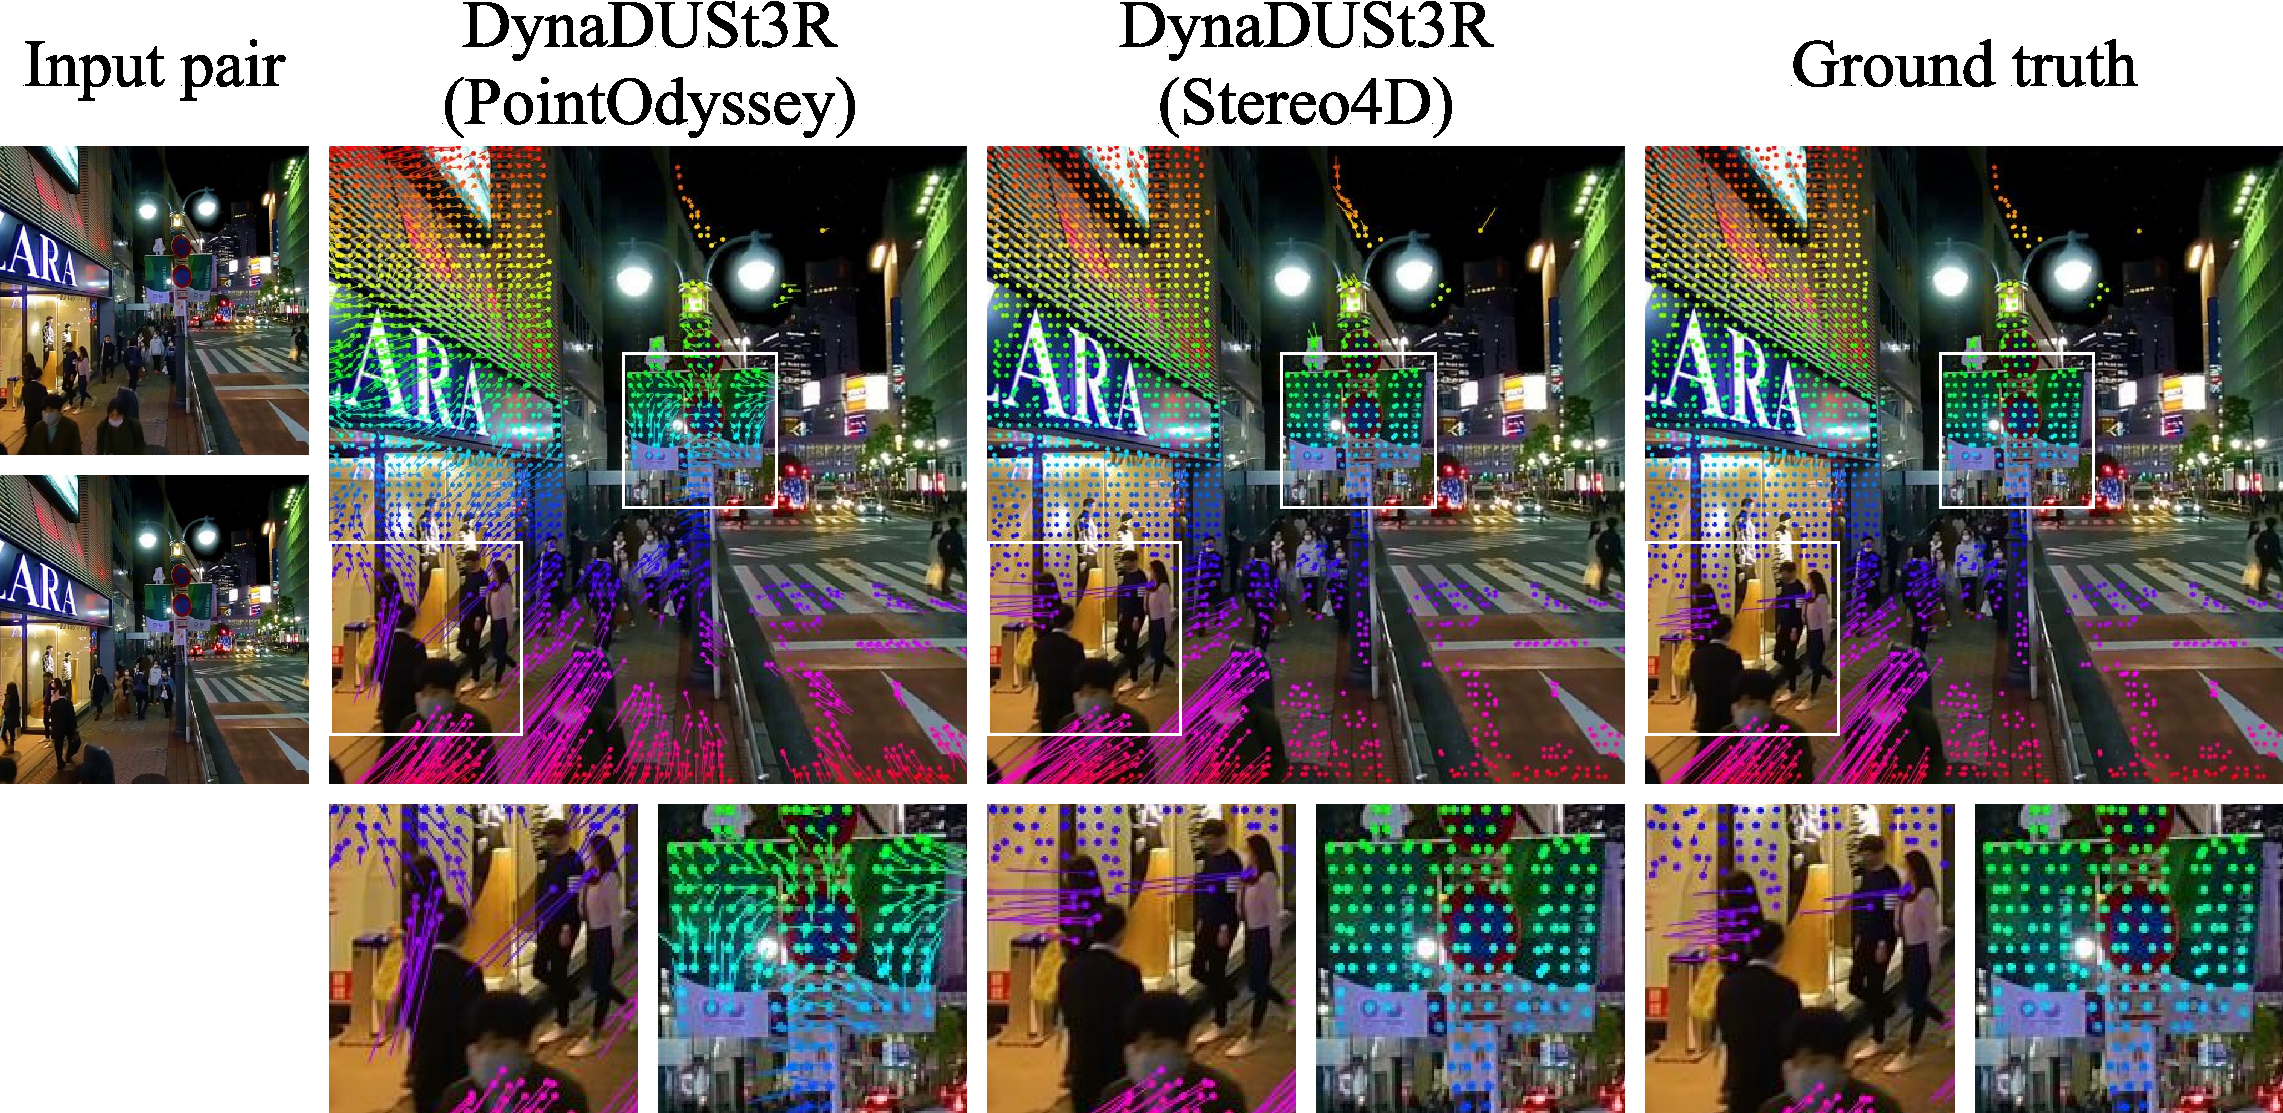
\includegraphics[width=\linewidth]{fig/qualitative_comparison_on_motion_stereo4d.pdf}
    \caption{\textbf{Qualitative comparisons, 3D motion on the \dataset.} We compare variants of DynaDUSt3R trained on different data sources. The PointOdyssey-trained model incorrectly predicts significant 3D motion on static elements such as the building wall and the banners near the streetlight, while the Stereo4D-trained model correctly predicts these elements as stationary. The Stereo4D model also makes more precise motion predictions for dynamic objects, such as humans with large movements (bottom row).}
    \label{fig:compare-stereo4d}
\end{figure}

\bfpar{Quantitative results.}
We show numerical results for two-frame 3D motion prediction 
in \Tab{motion_3d_eval}. 
\method trained on real-world data achieves better generalization and outperforms the baseline trained on PointOdyssey significantly across all 
metrics. This suggests the potential of our data for more effective learning of real-world 3D motion priors.



\begin{figure}[ht]
    \centering
    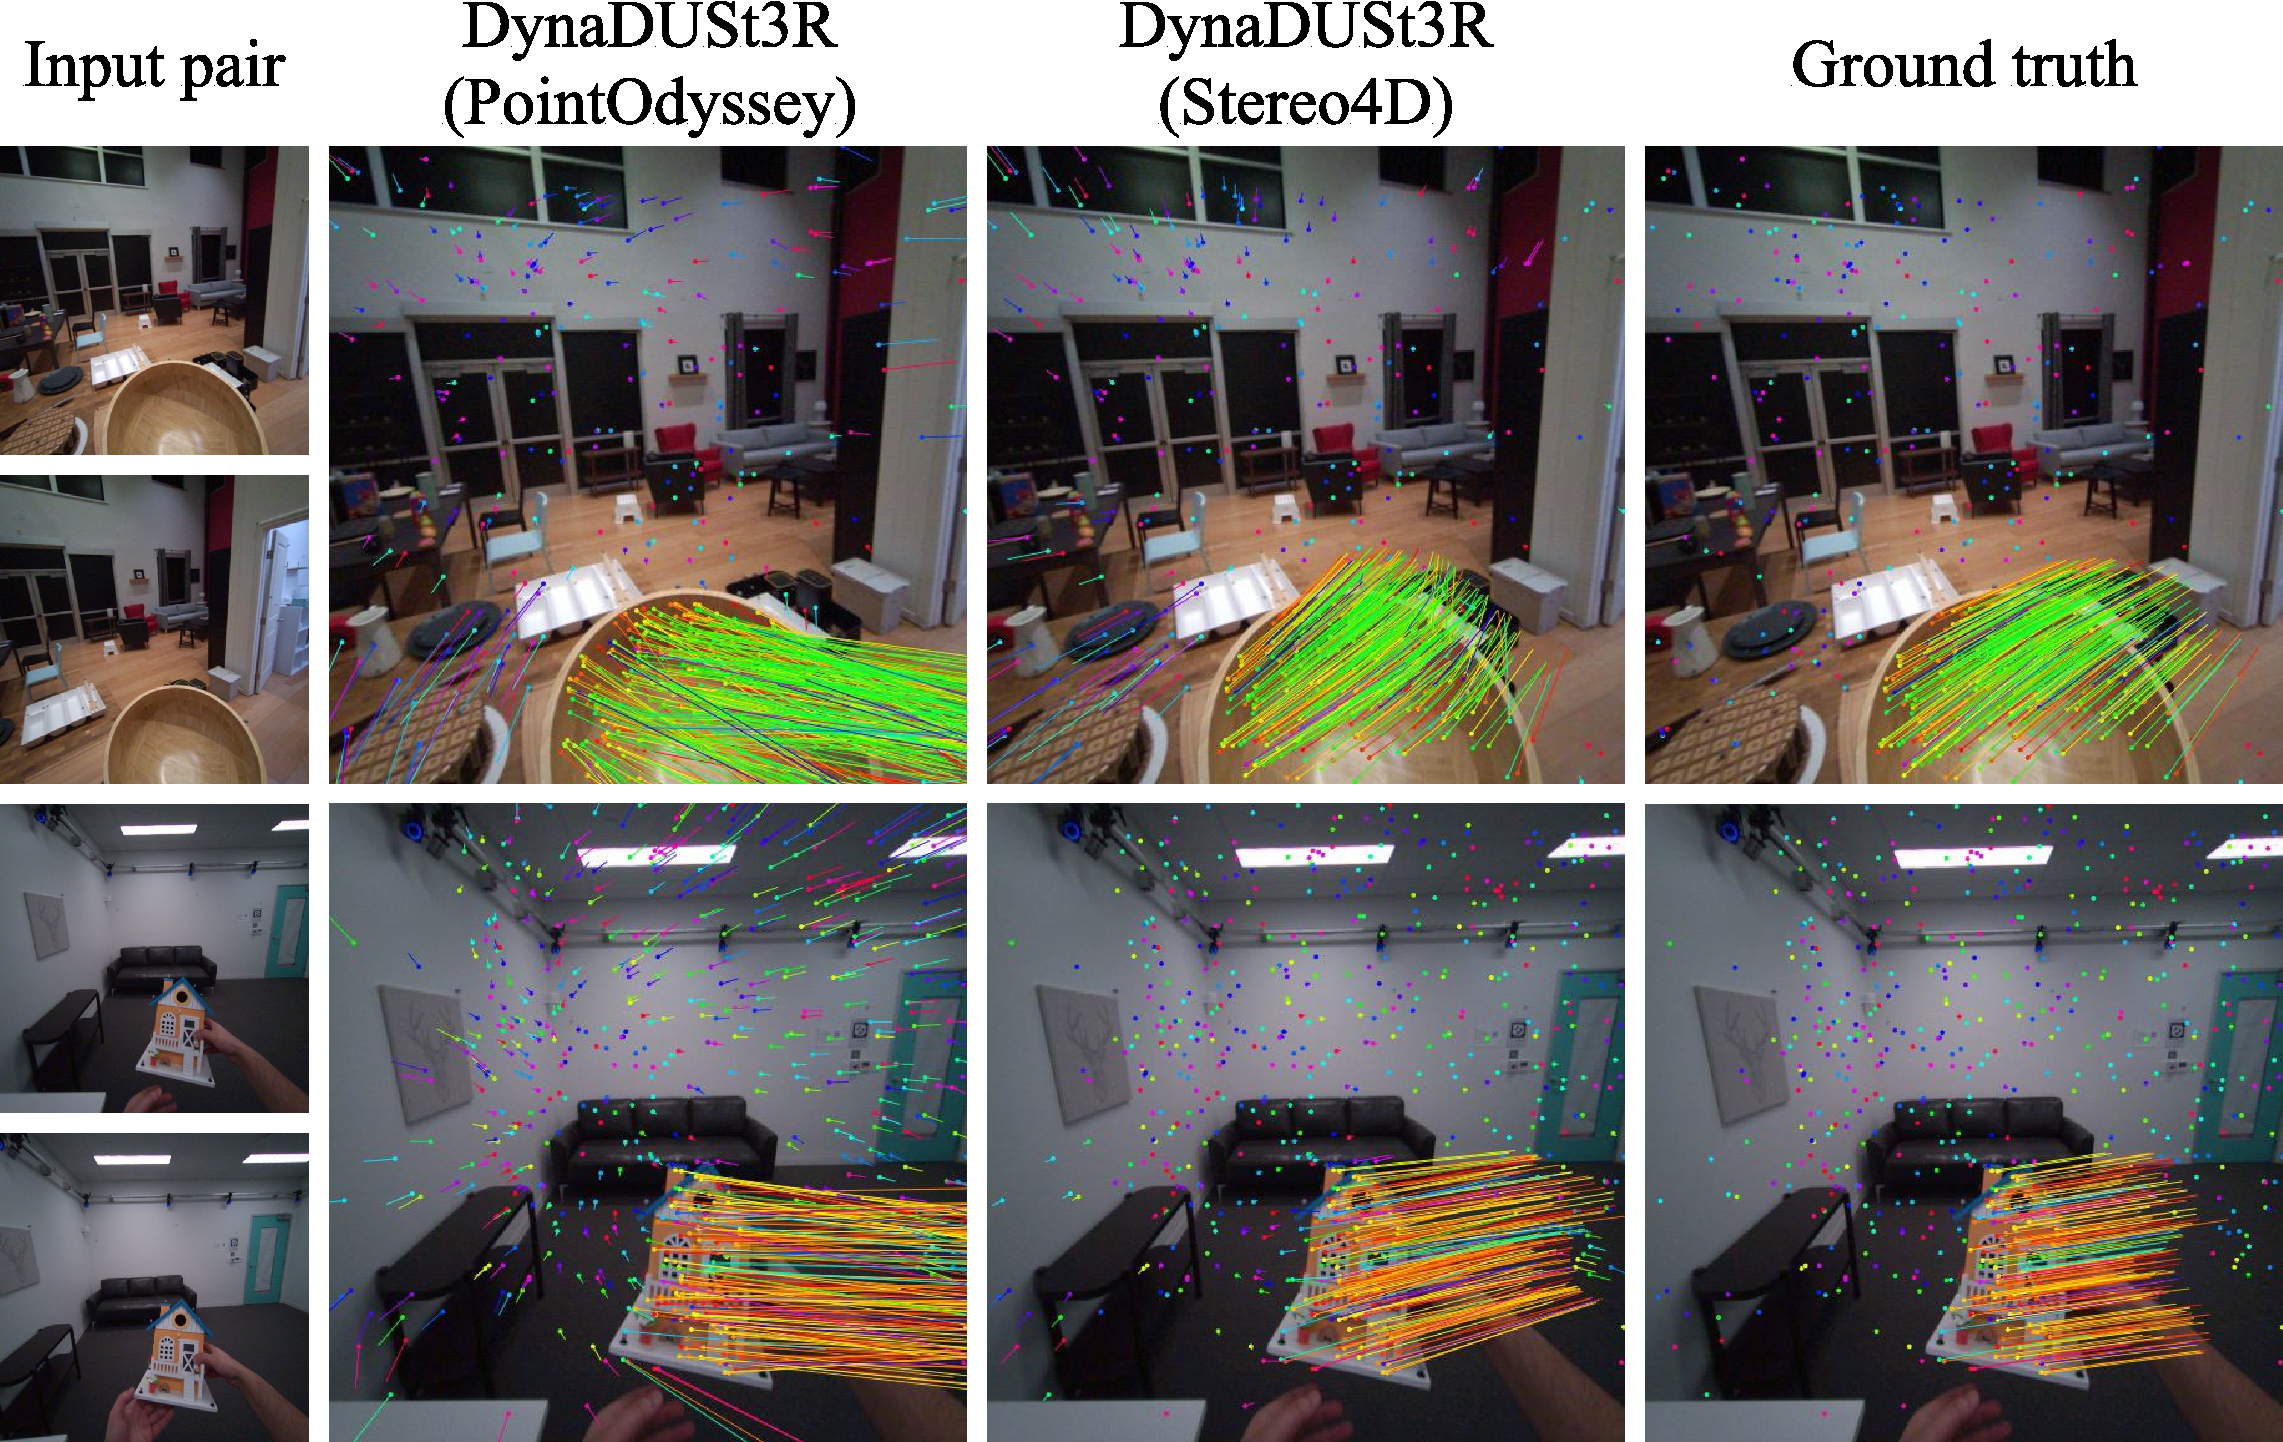
\includegraphics[width=\linewidth]{fig/tapvid3d_adt.pdf}
    \caption{\textbf{Qualitative comparisons of predicted 3D motion on ADT~\cite{pan2023aria}.} \method trained on \dataset produces more accurate 3D motion compared to training on PointOdyssey.} %
    \label{fig:compare-stereo4d-adt}
\end{figure}

\bfpar{Qualitative results.}
\Fig{result-wall-stereo4dtest} shows example results for three dynamic scenes in our \dataset test set, including visualizations of 3D point clouds and motion tracks.
\method produces accurate 3D shape and motion tracks over the timespan defined by the two input images. Despite the inputs being two sparse images, our architecture enables querying intermediate motion states, resulting in continuous and potentially non-linear motion trajectories.%

We also qualitatively compare predicted 3D motion tracks between \method networks trained on \dataset and on PointOdyssey, by projecting their predicted 3D motion vectors into 2D image space.
\Fig{compare-stereo4d} and \Fig{compare-stereo4d-adt} show comparisons on the \dataset and ADT test set respectively. \method trained on \dataset produces more accurate 3D motion estimates for both static and moving objects. For instance, \method trained on PointOdyssey produces non-zero motion for the stationary street banner and erroneous motions for the walking people in \Fig{compare-stereo4d}.










\begin{figure*}[ht]
    \centering
    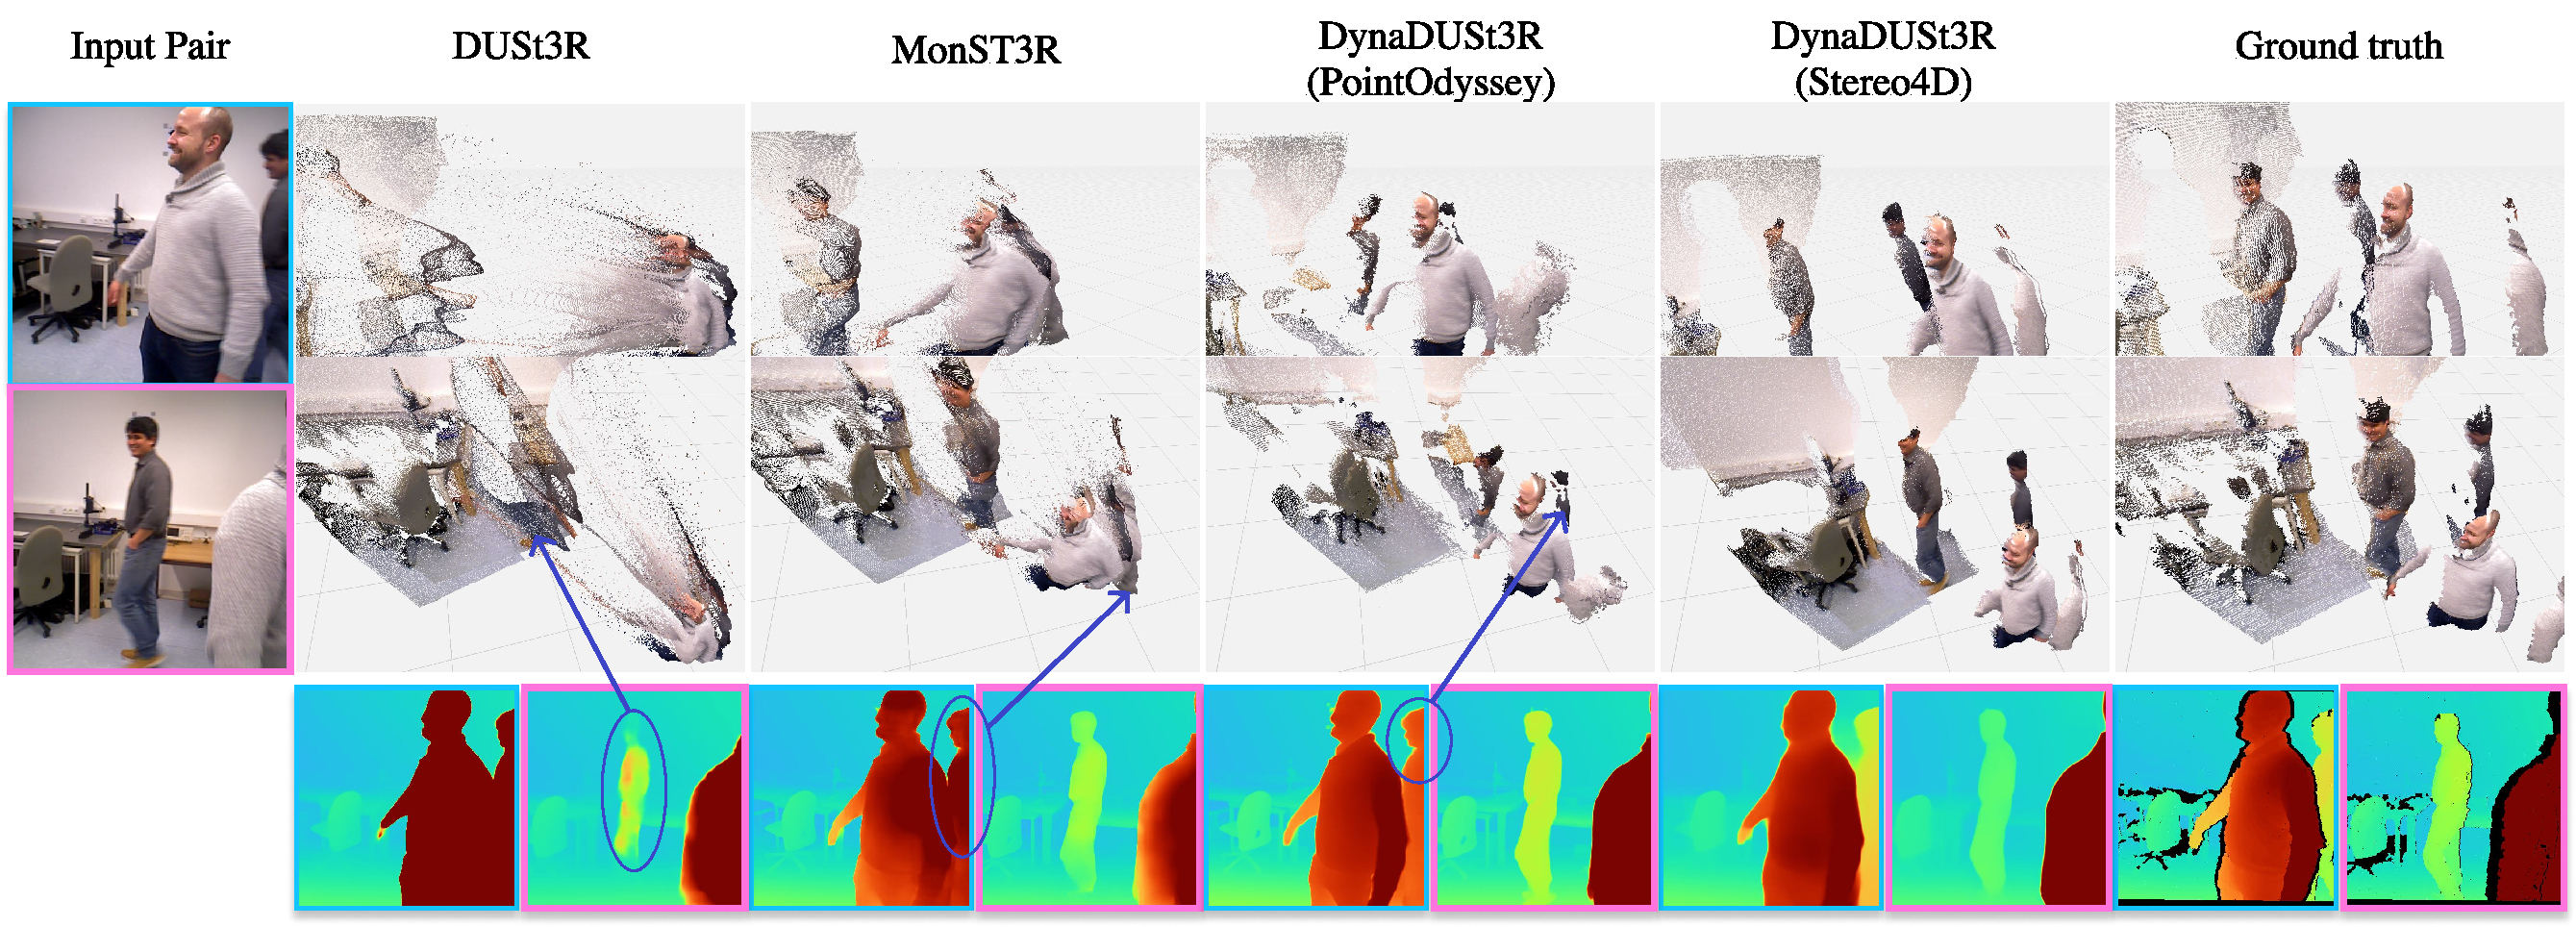
\includegraphics[width=\linewidth]{fig/depth_comparison.pdf}
    \caption{\textbf{Qualitative comparison, 3D structure on Bonn~\cite{palazzolo2019iros}.}  From left to right, we show an input image pair, predictions from different methods, and the ground truth geometry. 
    The top two rows show 3D point clouds from two viewpoints, where we show the union of the pointmaps for the two input time steps. The bottom row shows the corresponding disparity for two input images. 
    Compared to all the other methods, \method trained on \dataset achieves better 3D structure predictions with finer details.}
    \label{fig:compare-bonn}
\end{figure*}

\subsection{Structure prediction} \label{sec:structure_eval}
\noindent \textbf{Baseline and metrics.}
We evaluate the quality of predicted 3D structure by comparing depth maps predicted by \duster~\cite{wang2024dust3r}, MonST3R~\cite{zhang2024monst3r}, and \method trained on \dataset or PointOdyssey. 
\duster is designed to predict aligned point clouds from two input images of a static scene.
MonST3R, a concurrent approach, extends \duster to handle dynamic scenes by predicting time-varying point clouds without modeling motion.

We evaluate predicted depth accuracy on the Bonn~\cite{palazzolo2019iros} dataset and our held-out test set, where we sample two views that are 30 frames apart from a video. 
Since we focus on the two-frame case, we do not apply any post-optimization to the network outputs.
In addition, since all methods predict 3D point clouds in the coordinate frame of the first image, we include the two points clouds predicted from both input frames in our evaluation. We use standard depth metrics, including absolute relative error (Abs Rel) and percentage of inlier points $\delta<1.25$, following prior work~\cite{NVDS, zhang2024monst3r}.  We use the same median alignment as before to align the predicted depth map with the ground truth.

\bfpar{Quantitative comparisons.}
We show quantitative comparisons of depth predicted by different methods in \Tab{depth_eval}. \method trained on \dataset outperforms all other baselines by a large margin. In particular, we demonstrate improved depth prediction on the unseen Bonn dataset.

\bfpar{Qualitative comparisons.}
We provide additional visual comparisons in \Fig{compare-bonn}, where we visualize ground truth 3D point clouds and predictions from our approach and the other three baselines at different input time steps. DuST3R predicts inaccurate depth relationships for the two moving people, while MonsT3R and \method trained on PointOdyssey both predict distorted scene geometry. In contrast, our model trained on \dataset produces 3D structure that most closely resembles the ground truth.







\begin{table}[!t]
\centering
\footnotesize
\renewcommand{\arraystretch}{0.95}
\renewcommand{\tabcolsep}{2.pt}

\resizebox{\linewidth}{!}{
\begin{tabular}{@{}lcccc@{}}
\toprule
  & \multicolumn{2}{c}{Stereo4D} & \multicolumn{2}{c}{Bonn~\cite{palazzolo2019iros}}  \\ 
 
\cmidrule(lr){2-3} \cmidrule(lr){4-5}
 Method & Abs Rel$\downarrow$ &$\delta<1.25$$\uparrow$ &Abs Rel$\downarrow$ &$\delta<1.25$$\uparrow$  \\ 
\midrule
\duster~\cite{wang2024dust3r} &0.2696 & 67.77 & 0.1098& 84.93 \\
\monster~\cite{zhang2024monst3r} &0.1939 & 72.56 & 0.0721&92.60\\
Ours (PtOdyssey) & 0.3858 & 61.87 & 0.0691 &95.94\\ 
Ours (\dataset) &\textbf{0.1032} & \textbf{87.93} & \textbf{0.0653} & \textbf{96.02} \\ 
\bottomrule
\end{tabular}
} 

\caption{{\bf Quantitative comparison, depth maps.} \method trained on our \dataset data surpasses the performance of the model trained on PointOdyssey~\cite{zheng2023point}, as well as \duster and \monster under challenging sparse view settings.
}\label{tab:depth_eval}
\end{table}



